\input{~/Documents/LatexPresets/programming/preambule.tex}
%\usepackage{mathtools}
%\usepackage{amssymb}
\usepackage{hyperref}
\usepackage[perpage,bottom]{footmisc}

\newcommand{\basedir}{~/FESB/2. semestar/3D Simulacije/Izvještaji/vjezba6}
\title{Vježba L05}
\author{Jakov Spahija}

\begin{document}
\maketitle
\vspace{15em}
\tableofcontents
\pagebreak

%%%%%%%%%%%%%%%%%%%%%%%%%%%%%%%%%%%%%%%%%%%%%%%%%%%%%%%%%%%%%%%%%%%%%%%%%%%
\section{Prazan VanityXS projekt}
\label{sec:UWP}
\setcounter{lstlisting}{0}

%\begin{codesection}
%	\lstinputlisting[style=C++,numbers=none,firstline=10,lastline=14,caption=\_\_vectorcall konvencija]{\basedir/DXM Vectors/Functions.h}
%\end{codesection}

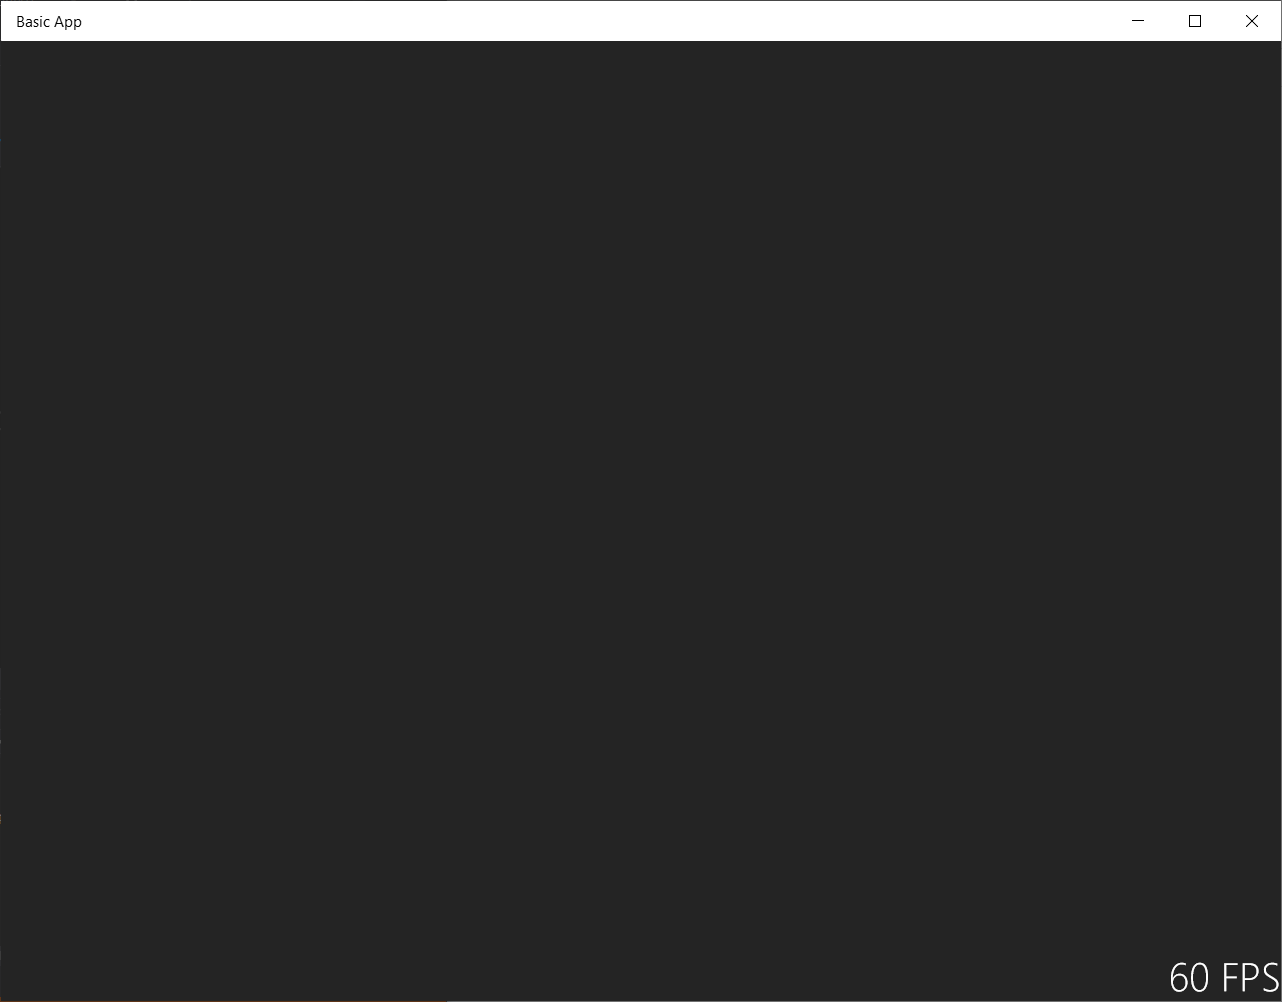
\includegraphics[width=450px]{..\\window.png}

\vspace{3em}
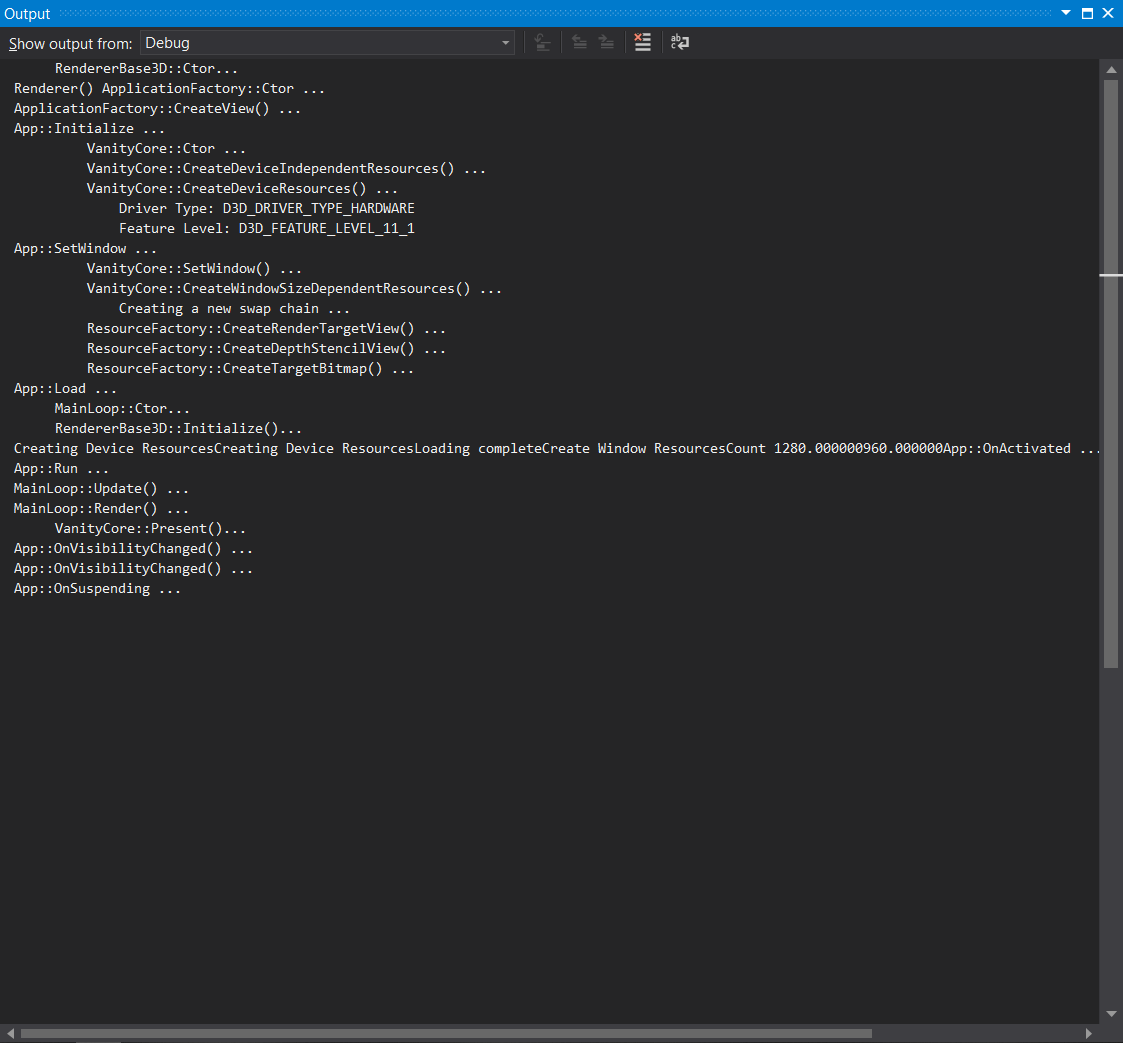
\includegraphics[width=450px]{..\\OutputDebug.png}

\pagebreak

\end{document}
